\documentclass[12pt]{book} 

\usepackage{amsmath}
\usepackage{graphicx}
\usepackage{import}
\usepackage{amsfonts}
\usepackage{booktabs}

\setlength{\parindent}{0em}  % sets auto indent at new paragraph to none

\newcommand{\incfig}[1]{%
        \import{./figures/}{#1.pdf_tex}
}

\newcommand{\und}{%
        \underline
}

\newcommand{\incimg}[2]{%
       \begin{figure}[h]
               \centering
               \includegraphics[scale = #2]{./figures/#1}
       \end{figure}
}

\title{\coursetitle\linebreak\lecturename}
\author{\\Cain Susko\\ 
           \\ \\ \\
      Queen's University 
    \\School of Computing\\} 

%=-=-=-=-=-title-=-=-=-=-=%
\newcommand{\lecturename}{Nonlinear Separation}
\newcommand{\coursetitle}{Linear Data Analysis}
%=-=-=-=-=-#####-=-=-=-=-=%

\begin{document}
\begin{titlepage}
        \maketitle
\end{titlepage}


\section*{a High Dimensional PCA}
the main concept of this lecture is how one can perform a PCA on higher
dimension data as well as how to avoid directly embedding 
vectors using the Gram matrix. It will also cover the derivation and 
algorithm for kernel PCA. 

\section*{b Scatter Matrix of Observations}
Given the data: $A \in \mathbb{R}^{m \times n}$, we can find the 
zero mean matrix as:
\begin{align*}
        M &= A - \vec 1\bar A\\
          &= [I-\frac{1}{m}\vec 1 \vec 1^\top]A\\
          &= G_mA
\end{align*}

Where $I$ is the identity matrix and $G$ is called the centring.
\paragraph{Style (1)}
Therefore, the scatter matrix is:
\[S_v = M^\top M\]

If we then write $M$ as $M = V\Sigma^\top\Sigma V^\top$, then $S_v$ equals:
\[S_v = V\Lambda_v V^\top\]

\paragraph{Style (2)}
Given: $S_u = MM^\top$, we can expand to:
\[S_u = U\Sigma\Sigma^\top U^\top\]
which simplifies to be:
\[S_u = U\Lambda_u U^\top\]

\subsection*{Scoring}
The above examples show the column (1) and row (2) form of the scatter
matrix. Because the rank of $M$ equals $r$, this implies the
first $r$ eigenvalues in the variable style $\Lambda_v$ and observation 
style $\Lambda_u$ are equal !!! Therefore, in order to score either 
style one can use a single equation:
\[Z = U\Lambda^{\frac{1}{2}}\]

We can also rewrite $S_u$ using the centring matrix such that:
\begin{align*}
        S_u &= MM^\top\\
            &= G_mAA^\top G_m^\top
\end{align*}

\section*{c Kernel PCA Using The Gram Matrix}
Given $m$ observations, embed $\und a_j \hookrightarrow \hat a_j$.
\[\hat S_u \in \mathbb{R}^{P \times P}\]

Recall, the Gram matrix $\hat W \in \mathbb{R}$ is square, 
symmetric, and positive semi-definite. It's entries
are:
\[\hat W_{i,j} =^{def} k(\und a_i, \und a_j)\]

Therefore, the scatter matrix would be:
\begin{align*}
        \hat S_u &= G_m[\hat A\hat A^\top]G^\top_m\\
                 &= G_m\hat WG_m^\top
\end{align*}

This means we will never need to embed vectors, instead we 
will compute each entry of $\hat W$ using the kernel function.

\subsection*{Kernel PCA}
after computing $\hat S_u = \hat U\hat\Lambda\hat U^\top$ (notation 
changed for ease of understanding), we then perform PCA which 
we can use to find the score:
\[\hat Z = \hat U\hat\Sigma\]

This kernel PCA is slower than PCA as there are normally many more 
observations than variables.
\pagebreak

\section*{d Kernel PCA on Iris Data}
There will be 2 examples; One for conventional PCA and one for Kernel
PCA. They will both use k-means to cluster and the kernel being used
in kernel PCA is Gaussian with $\sigma^2 = m = 150$
\begin{itemize}
        \item[\textbf{Conventional}] after reducing and scoring the
                data the kmeans plot is:
                \begin{figure}[h]
                        \centering
                        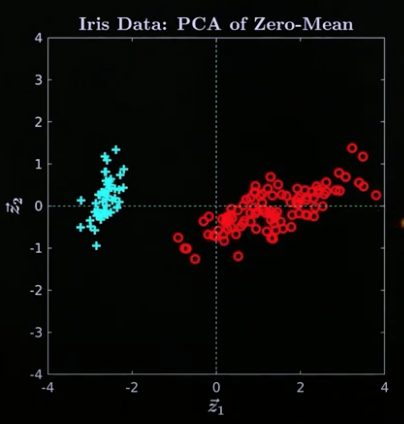
\includegraphics[scale=0.4]{./figures/data1}
                        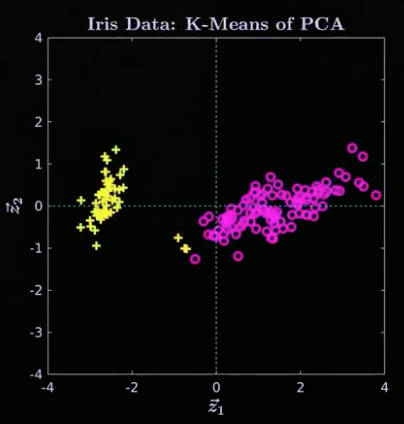
\includegraphics[scale=0.4]{./figures/kmean1}
                \end{figure}

                Which is an ok--but not great seperation (outliers)
        \item[\textbf{Kernel}] Kernel PCA resulted in:
                \begin{figure}[h]
                        \centering
                        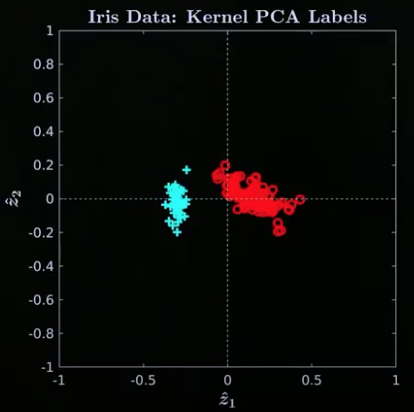
\includegraphics[scale=0.4]{./figures/data2}
                        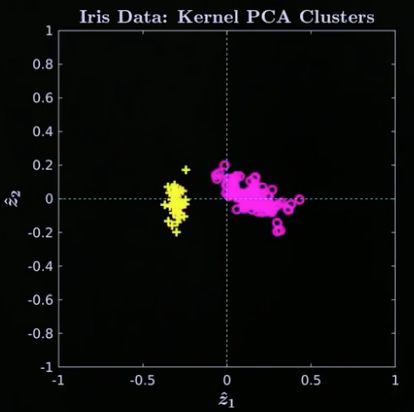
\includegraphics[scale=0.4]{./figures/kmean2}
                \end{figure}

                which is a much more accurate separation of
                the data.
\end{itemize}

\section*{Learning Outcomes}
Students should now be able to:
\begin{itemize}
        \item compute a Gram matrix from given data
        \item using the centring matrix to center Gram matrix
                for PCA
        \item compute scores for Kernel PCA
        \item assess the results for simple data
\end{itemize}

\end{document}
